\documentclass[a4paper, 11pt]{article}
\usepackage{comment} % enables the use of multi-line comments (\ifx \fi) 
\usepackage{fullpage} % changes the margin
\usepackage{pdflscape}
\usepackage{rotating}
\usepackage{graphicx}
\usepackage[table]{xcolor}

\begin{document}
%Header-Make sure you update this information!!!!
\noindent
\large\textbf{Program Assignment 2} \hfill \textbf{Longxiang Li} \\
\normalsize CS124 \hfill Teammates: No \\

\section*{Introduction}
Strassen's matrix multiplication algorithms works faster for $n$ by $n$ matrix than the conventional naive algorithm whose time complexity is $O(n^3)$, in theory. However, for some smaller n, the conventional algorithm runs faster because the time consumed in memory allocation in Strassen's algorithm. But, for this recursive algorithm, we don't need to go to the basic element of this matrix (a $1\times1$). We may modified the classic algorithm by converting from recursion to conventional algorithm when the dimension is small enough. We call this cross-over point. In this experiment, we try to find the optimal cross-over point for different $n$ from two direction. First, we calculate the exact running time for Strassen's algorithm, modified Strassen's algorithm and conventional algorithm and estimate the cross-over point numerically. These calculation were based on the assumption that the cost of any single arithmetic operation is 1 and all others are free. Second, we implemented these algorithms and get the cross-over point in practice.
\section*{Numerical Analysis of cross-over point}
To simplify the calculation we assume in the following analysis in this section, the dimension n is power of 2 and the cross-over value is also power of 2. In classic Strassen's algorithm, for a given matrix of given $n$, we require 7 multiplication of matrices of simension $\frac{n}{2}$. In addition, there are 18 summation and subtraction of size $\frac{n}{2}$. Thus, we can write a recursive equation of the running time:
\[{f_1}(n)=7f(\frac{n}{2})+18(\frac{n}{2})^2\] 
\[=7^2f(\frac{n}{4})+7\times18 (\frac{n}{4})^2+18(\frac{n}{2})^2\] 
\[=7^kf(\frac{n}{2^k})+18n^2\{7^{k-1}(\frac{1}{2^k})^2+\dots+7^0(\frac{1}{2})^2\}\]
when $k=log_2{n}$, we arrive at the basic case. Since $f(1)=1$. We can conclude that the exact running time of standard Strassen's algorithm is:
\[f_s(n)=7^{log_2{n}}+6n^2\{(\frac{7}{4})^{log_2{n}}-1\}\]
For conventional algorithm, we have a total of $n^3$ multiplication and $n^2(n-1)$ additions. So the close form running time of conventional algorithm is:
\[f_c(n)=n^2(2n-1)\]
Let's assume we set cross-over point at $n_0$. That means above $n_0$, we used Strassen's algorithm and below $n_0$, we used conventional algorithm. So the running time of this hybrid algorithm is:
\[f_{n_0}=7^{log_2{\frac{n}{n_0}}}(2n_0^3-n_0^2)+6n^2((\frac{7}{4})^{log_2{\frac{n}{n_0}}}-1)\]

We cannot achieve a closed form $n_0$ for every $n$. But we can get a numeric estimation. The theoretical running time of standard Strassen's, modified Strassen's with $2\times2$, $4\times4$, $8 \times 8$, $16 \times 16$ basic matrix and conventional algorithm are listed below:
\begin{table}[ht]
	\centering
	\begin{tabular}{rrrrrrrr}
		\hline
		& n & Strassen's & 2*2 & 4*4 & 8*8 & 16*16 & Conventional \\ 
		\hline
		 & 16 & 15271 & 10812 & 8656 &\cellcolor{blue!25} 7872 & 7936 & 7936 \\ 
	 & 32 & 111505 & 80292 & 65200 &\cellcolor{blue!25}  59712 & 60160 & 64512 \\ 
		& 64 & 798967 & 580476 & 474832 &\cellcolor{blue!25}  436416 & 439552 & 520192 \\ 
		 & 128 & 5666497 & 4137060 & 3397552 &\cellcolor{blue!25}  3128640 & 3150592 & 4177920 \\ 
		 & 256 & 39960391 & 29254332 & 24077776 &\cellcolor{blue!25}  22195392 & 22349056 & 33488896 \\ 
		 & 512 & 280902385 & 205959972 & 169724080 &\cellcolor{blue!25}  156547392 & 157623040 & 268173312 \\ 
		 & 1024 & 1971035287 & 1446438396 & 1192787152 &\cellcolor{blue!25}  1100550336 & 1108079872 & 2146435072 \\ 
		\hline
	\end{tabular}
\end{table}
For a matrix with size of $n$, when $n\leq 16$, by no means can Strassen's run faster than conventional algorithm in theory. However, if we chose a cross-over point at 8, the modified Strassen's algorithm consume fewer calculation operation than the conventional algorithm. This is true for other matrix dimension. Because if the dimension of a matrix is a power of 2, the cross-over points should also be powers of 2. So, at least when $n<2^12$, $n_0=8$ according to numeric analysis.
In this plot, we could find the cross-over point is located at $8\times8$ for both matrix size of 4096 and matrix size of 256.
\begin{figure*}[h]
	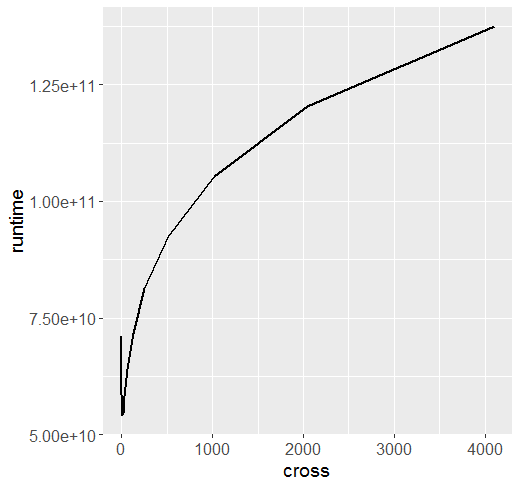
\includegraphics[width=0.5\linewidth]{Truntime}
	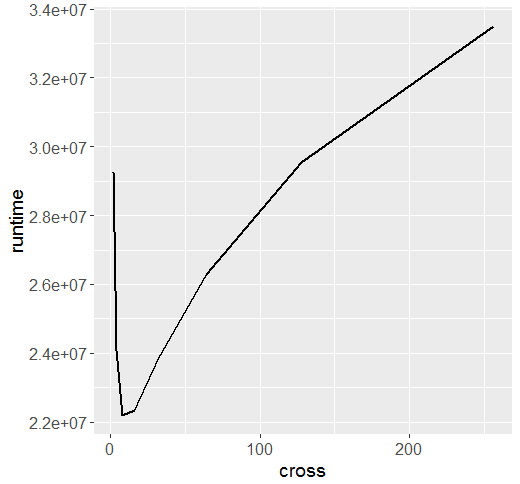
\includegraphics[width=0.5\linewidth]{Truntime8}
	\caption{Theoretical runtime of matrix multiplication by modified Strassen's algorithm of different cross-over points}
	\label{fig:truntime}
\end{figure*}

\section*{Implementation}
Our implementation was straightforward, similar with given in class.

 First, We created utility functions matrix sum, matrix subtract, matrix initiation and matrix release. Then we implement the conventional algorithm. According to the hint, there's a performance difference between column first implementation and row first implementation. We found that column first implementation ran faster. So this implementation was applied here. Subsequently, we implemented the Strassen's algorithm. To begin with, we created a function to divide our matrix into four sub-matrix equally. After splitting, we utilized the functions created above to implement the addition and multiplication. Finally, the four sub-matrix were merged as output. After doing these calculation, all memories were released.

However, this implementation only works when dimension is a power of 2, indicating the dimension can be divided by 2 recursively. In our dimension, when the dimension is odd, we tab one row of zeros at the bottom and one column of zero at right end to make the dimension dividable by 2 again. This is very different from tabbing zeros to the extent that the new dimension is a power of 2. After running a standard Strassen's on this extented matrix, we extract the left-upper $n*n$ elements as output.We tested this algorithm in experiment and proved this is correct by comparing with conventional algorithm's result.

\section*{Experimental analysis of cross-over point}

\section*{Final Evaluation}

\section*{Attachments}
\end{document}
